%!TEX root = ../main.tex

\graphicspath{{./figures/introduction/}}

\chapter{FISH-based transcriptomics}
\label{ch:introduction}

\minitoc
\newpage

In this introduction, I will present the gene expression process in order to describe the biological context where \ac{RNA} localization happens.
Then, I will present the experimental protocols that allows us to visualize and analyse \ac{RNA} molecules as well as the machine learning tools I applied.
I will finish this introduction with an overview of my thesis goals, a list of the contributions I made and a summary of this manuscript to guide the reader.

\section{Gene expression process}
\label{sec:gene_expression}

Cells are the basic unit of all living organisms.
Yet, a diversity of cell-type exists, performing different actions.
Some of those are common among all cells (cell division for example), but others can be very specific.
Most of the time, different cell-types perform diverse actions through a different set of functional molecules.
In order to implement these different cellular processes and to fulfill the variety of diverse functions, a cell gets its instructions from the \ac{DNA}.
The latter contains all the cell's genetic information and it is common for all cells of the same organism.
A \ac{DNA} strand presents a succession of genes, defined as long sequences of nucleotides.
They are organics molecules composed of a five-carbon sugar, a phosphate group and one of the four nucleobases: Adenine, Cytosine, Guanine and Thymine.
Together, these nucleobases form a genetic alphabet of 4 letters (A, C, G and  T).
Each gene encodes the blueprint of a functional molecule with a specific sequence of nucleobases.

Gene expression is the process by which genetic information is transformed into functional products.
\ac{RNA} molecules, or transcripts, are essential for this process.
They are either the functional gene products themselves or they serve as an intermediate molecule prior to the production of other functional products, namely the proteins.
A change in gene expression gives cells enough flexibility to adapt and react to different external stimuli.
It also drives cells differentiation, allows them to run their basic functions, modulate their activities and therefore appears to be one of the most fundamental processes of life.
On the contrary, its deregulation can lead to various diseases.
This explains the interest of the scientific community to study and decode gene expression processes.

In the living world, cells can be divided in two categories: prokaryotic cells and eukaryotic cells.
The prokaryotic cells, which do not have a nucleus and typically form a unicellular organism, and the eukaryotic cells, with a well-organized nucleus.
An eukaryote (a living organism with eukaryotic cells) is usually composed of cells with a higher level of compartmentalization through membrane-bound organelles.
The nucleus is obviously the most important of these organelles, with the \ac{DNA} inside.
The rest of the organelles are located in the cytoplasm, such as the mitochondria, the lysosomes, or the Golgi apparatus (see Figure~\ref{fig:eukaryotic_cell}).

For an eukaryote cell, the expression of a gene includes two main steps: the transcription of a \ac{DNA} sequence into a \ac{RNA} (in the nucleus) and the translation of a \ac{RNA} into a protein.
Between these two major steps, there is a phase of maturation for the transcript, before a potential exports outside the nucleus and a transport somewhere in the cytoplasm.
A cell can regulate either the transcription or the translation step to control the production of its functional molecules and thereby the biological process to which the proteins or \ac{RNA} contribute\footnote{For a complete and general introduction about cellular biology, an interested reader could see~\cite{alberts_molecular_2017}.}.

\begin{figure}[]
    \centering
    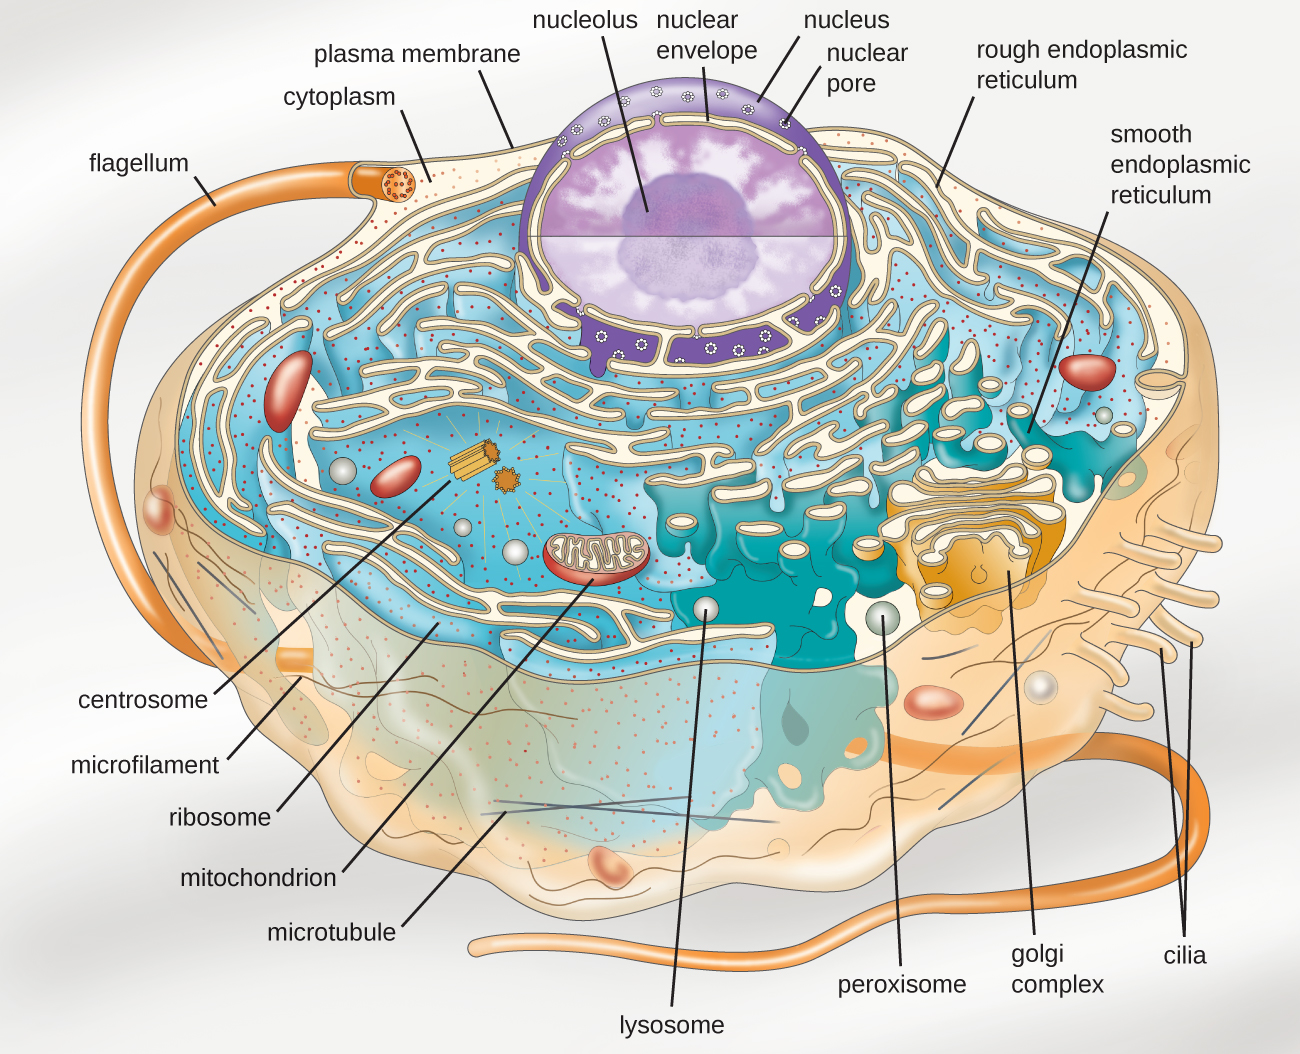
\includegraphics[width=0.8\textwidth]{figures/introduction/cell_eukaryotic.jpg}
    \caption[Illustration of an eukaryotic cell]{Illustration of an eukaryotic cell, from~\cite{parker2017microbiology}}
    \label{fig:eukaryotic_cell}
\end{figure}

\subsection{Transcription}
\label{subsec:intro_transcription}

\subsubsection{The primary transcripts}

This step consists in copying a gene (a sequence of nucleotides along the \ac{DNA} strands) into another biomolecules composed of nucleotides: a \ac{RNA}.
While the \ac{DNA} is stuck within the nucleus, the \ac{RNA} can convey the blueprint of the future protein outside.
In many cases, \ac{RNA} can be non-coding (they do not lead to the synthesis of a protein) and fulfill a variety of functions itself, for instance the regulation of gene expression.
In a \ac{RNA}, the nucleotide Uracil (U) replaces the Thymine (T) and a ribose sugar serves as backbone instead of a desoxyribose sugar.
If both \ac{DNA} and \ac{RNA} contain genetic information, \ac{RNA} is a shorter single-stranded molecule, compared to the double-stranded \ac{DNA}, and, therefore, is less stable.
However, they both have two distinctive untranslated regions at their ends: 5'UTR and 3'UTR (corresponding to the number of carbon atoms in their sugar backbone extremities).\\

\noindent
Transcription proceeds as follows:
\begin{enumerate}
	\setlength\itemsep{0.1em}
	\item Proteins that serve as transcription factors bind to a specific sequence of \ac{DNA} (the promoter sequence) and recruit an enzyme (the \ac{RNA} polymerase) to initiate the transcription.
	\item The \ac{RNA} polymerase breaks the hydrogen bounds between the two \ac{DNA} strands to separate them.
	\item The \ac{RNA} polymerase moves along one \ac{DNA} strand, from 3' to 5' extremity, synthesizing a complementary nucleotides sequence on the way.
	\item The \ac{RNA} polymerase disengages from the strand when it meets a specific sequence of \ac{DNA} (the terminator sequence) and the newly synthesized nucleotides sequence (the primary transcribed \ac{RNA}) is released.
\end{enumerate}

\noindent
At this point, different sorts of \ac{RNA} are transcribed, depending of \ac{RNA} polymerase recruited:
\begin{itemize}
	\setlength\itemsep{0.1em}
	\item \ac{mRNA}, composed of coding (exon) and non-coding (intron) nucleotides, which conveys the blueprint of a future protein.
	\item \ac{rRNA} which, associated with ribosomal proteins, forms ribosomes, a macromolecular machine used by the cell to synthesize proteins.
	\item \ac{tRNA}, the most abundant \ac{RNA} molecule, which carries amino acids to the ribosome.
\end{itemize}

\begin{figure}[]
    \centering
    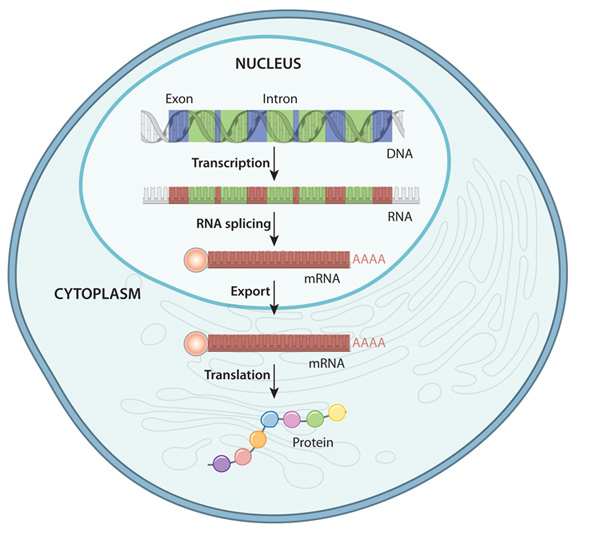
\includegraphics[width=0.8\textwidth]{figures/introduction/gene_expression_process.jpg}
    \caption[Schema of gene expression process]{Overview of gene expression process, from~\cite{cell_essential_nature}}
    \label{fig:gene_expression}
\end{figure}

\subsubsection{RNA maturation}

For the rest of the manuscript, I mainly focus on the \ac{mRNA}s.
They do not fit translation requirements yet and need to undergo three processes before leaving the nucleus:
\begin{itemize}
	\setlength\itemsep{0.1em}
	\item the 5' end is transformed (\ac{RNA} capping)
	\item a poly(A) tail (repeated adenine-based molecules) is added at the 3' end (polyadenylation)
	\item the non-coding parts of the \ac{RNA} sequence are removed (splicing)
\end{itemize}

\noindent
Those transformations enable to move the \ac{mRNA} out of the nucleus, regulate its degradation and promote the translation.
Figure~\ref{fig:gene_expression} shows a simplified illustration of the gene expression process.

\subsection{mRNA transport and localization}
\label{subsec:intro_rna_transport}

When an \ac{mRNA} is ready for export, it is moved out of the nucleus through the nuclear pore complex.
This complex recognizes a mature \ac{mRNA} if a specific set of proteins is bounded to it - poly(a) binding proteins, cap binding proteins, and proteins related to the splicing step.
Once in the cytoplasm, an \ac{mRNA} is not necessarily exploited by a ribosome for translation.
It can also be silenced by translational repressors and stored, transported in a specific region of the cell or degraded.

Until recently, the scientific community thought translation mostly occurred at the endoplasmic reticulum and then proteins were transported where they were needed.
New evidence suggests on the contrary that \ac{mRNA} localization within the cell is not always random and \ac{mRNA}s-proteins colocalization could be an important aspect of cell organization and gene expression regulation~\cite{lecuyer_global_2007}.
However, the involved mechanisms are not well understood yet and the extend of \ac{mRNA}s concerned by a specific localization pattern is still unknown.
Beyond the number of \ac{mRNA} molecules within a cell (the expression level of a gene), researchers manifest now an increasing interest for \ac{mRNA} localization~\cite{Chin_lecuyer_2017}.

\subsubsection{mRNA transport}

There is a specific sequence in the 3'UTR of the \ac{mRNA} molecule that acts like a \emph{zipcode}~\cite{Chabanon_2004}.
This sequence can be recognized by a \ac{RBP} and starts the formation of a \ac{RNP} complex.
This structure is then central to coordinate the transport, the translation and the degradation of the \ac{mRNA} molecule throughout the cell.\\

\noindent
Three mechanisms to transport \ac{mRNA} or locally enrich them are identified (see Figure~\ref{fig:rna_transport} for illustration):
\begin{enumerate}
	\setlength\itemsep{0.1em}
	\item Active transport of \ac{mRNA}s along the cytoskeleton, potentially coupled with an anchoring mechanism.
	This is the most common transport mechanism observed.
	Motor proteins are recruited by the \ac{RBP}s, bind to the \ac{mRNA} complex and transport it along actin filaments or microtubules.
	\item At specific places, \ac{mRNA} molecules are protected from degradation complexes.
	This localization is then locally enriched and the spatial distribution of the transcript is biased in favor of these protected localizations.
	\item Transcripts diffuse randomly across the cell, but local entrapment make them accumulate with an asymmetric distribution.
	This mechanism is notably observed in bacteria, where no active transport of \ac{RNA} has been observed~\cite{das_intracellular_2021}.
\end{enumerate}

\begin{figure}[]
    \centering
    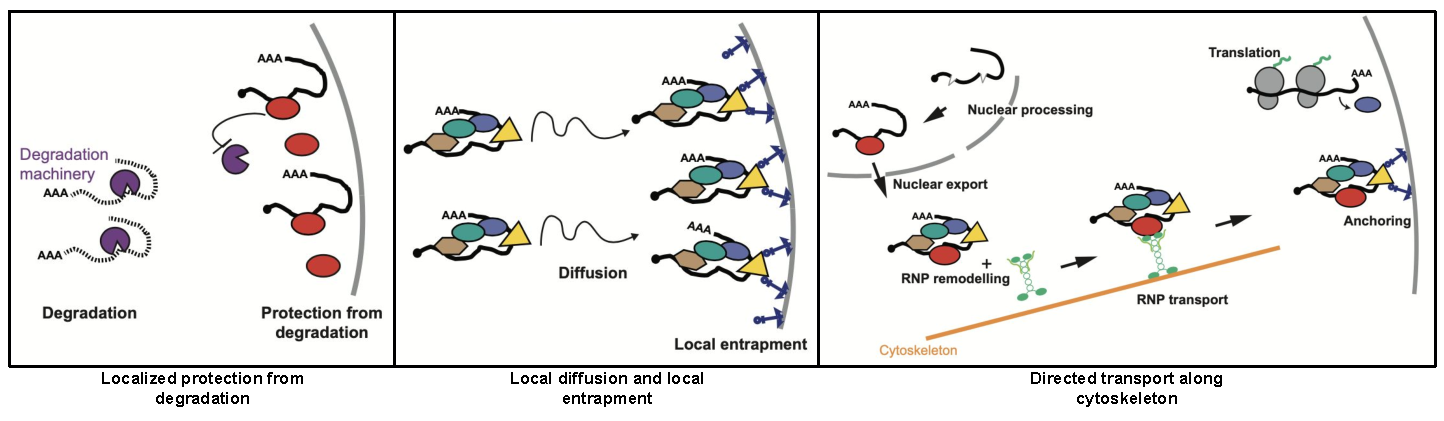
\includegraphics[width=\textwidth]{figures/introduction/rna_transport}
    \caption[Schema of RNA transport or locally enrichment mechanisms]{Schema of RNA transport or locally enrichment mechanisms, adapted from~\cite{Medioni_2012}.
	(\textit{Left}) RNAs are locally protected from degradation.
	(\textit{Center}) RNAs diffuse randomly, then they are locally entrapped.
	(\textit{Right}) RNAs are actively transported along cytoskeleton, thanks to RNP complexes and molecular motors.
	Directed transport can be coupled with an anchoring mechanism}
    \label{fig:rna_transport}
\end{figure}

\subsubsection{mRNA localization}

The localization of \ac{mRNA} can be see as an elegant and efficient mechanisms of regulation for the gene expression process.
By transporting one \ac{mRNA} molecule and promoting a local translation, several proteins can be directly produced at a desired place.
It saves the transport of a large amount of proteins~\cite{Medioni_2012}.
It also enables the cell to quickly react external stimuli.
This mechanism could be critical to modulate the synaptic plasticity in neuron cells for example~\cite{jung_axonal_2012}.
More generally, \ac{mRNA} localization will increase the cell compartmentalization and enable a higher flexibility and ''fine-tuning of gene expression in both space and time''~\cite{Medioni_2012}.

% mention Weeks et al. (1985) as first publication about RNA localization
% adham thesis: "Messenger localization was first discovered in Xenopus oocytes (Weeks et al., 1985)."

\subsection{Translation}
\label{subsec:intro_translation}

Finally, a cell synthesizes a protein through the translation process.
A ribosome is assembled around a \ac{mRNA} and moves along its nucleotides.
At the same time, \ac{tRNA}s carry amino acids matching the \ac{mRNA} sequence.
According to the genetic code, three successive nucleotides of the \ac{mRNA} (a codon) correspond to an amino acid.
The ribosome sequentially chains the amino acids, which then fold into a functional protein with a specific 3-dimensional structure.

\section{Imaging RNAs}
\label{sec:fish}

Our interest about \ac{RNA} localization requires advanced experimental protocol to analyze the \ac{RNA} subcellular distribution.
Traditional techniques are based on biochemical bulk-measurements, like microarrays~\cite{Schena_1995} or qRT-PCR~\cite{bustin_absolute_2000}.
They cannot operate at the single cell level and make the study of a spatial distribution within the cell impossible.
However, technical improvements are progressively addressing these limitations, for example with single cells \ac{RNA} sequencing~\cite{Hedlund_2018} or fluorescent in situ \ac{RNA} sequencing (FISSEQ)~\cite{Church_2014}.

An alternative option is to rely on images, which naturally provide the spatial insights and, with sufficient resolution, enable single cell analysis.
In addition, experiments should be scalable.
The design of large screens enables a systemic study of complex mechanisms and to cope with gene expression stochasticity, as well as heterogeneous \ac{RNA} distribution.

\begin{figure}[]
    \centering
    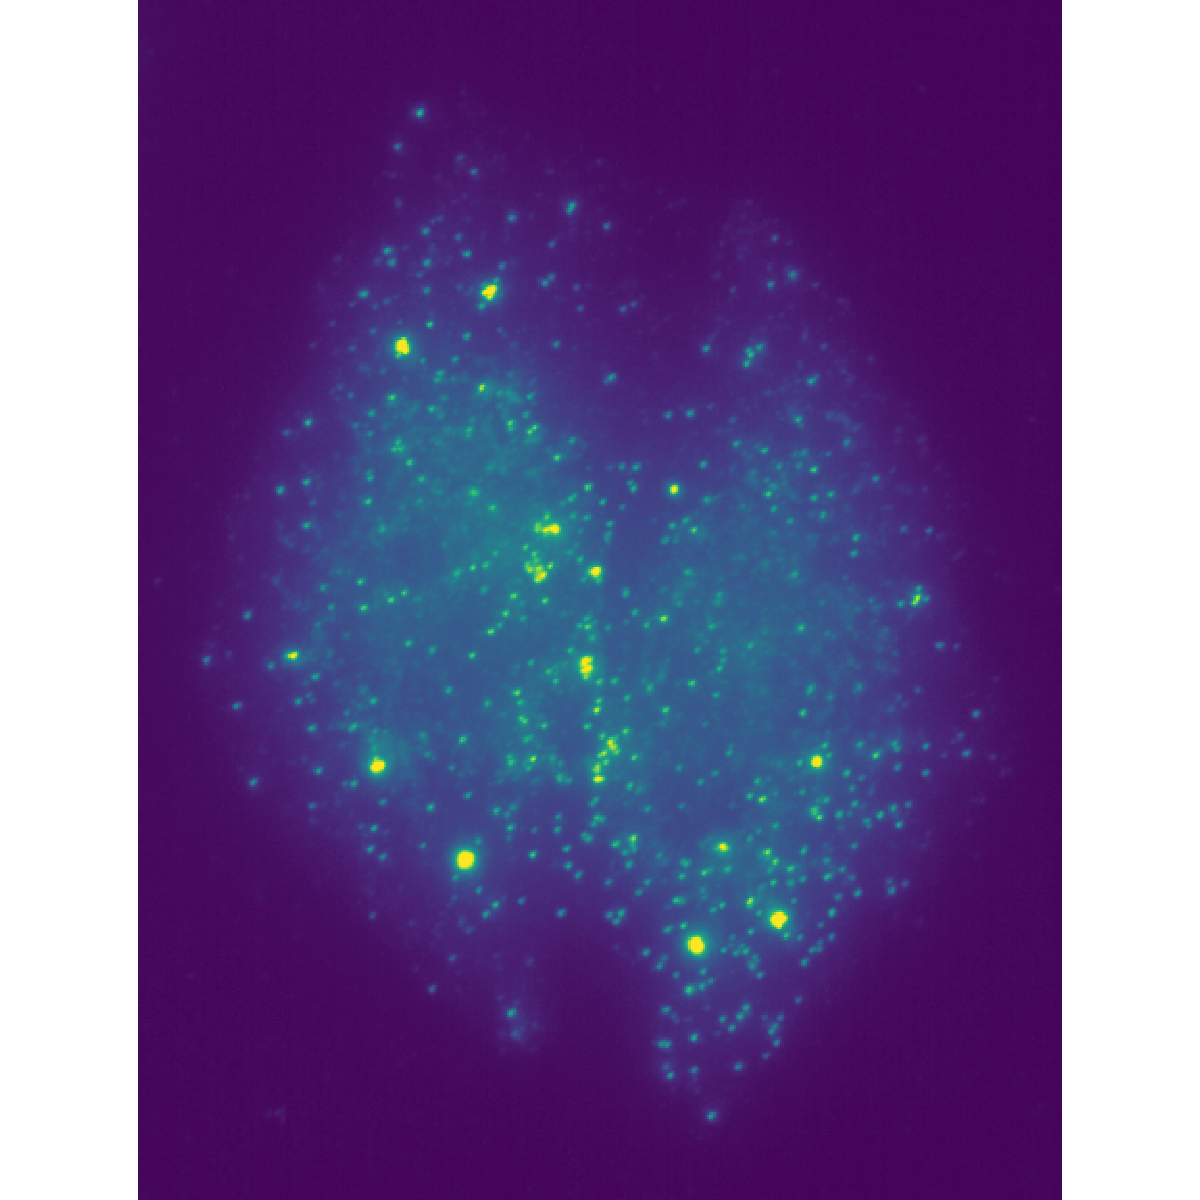
\includegraphics[width=0.7\textwidth]{figures/introduction/multichannel_input}
	\caption[Example of smiFISH image]{Example of smiFISH images with a maximum intensity projection.
	Each spot is a single RNA molecule}
    \label{fig:smFISH_input}
\end{figure}

\subsection{The smFISH experiment}
\label{subsec:intro_smfish}

Notably, \ac{smFISH} technique~\cite{Femino_1998}, is the first to reach single molecule resolution in fixed cells.
It uses multiple fluorescent oligonucleotides (or probes) to target and hybridize a transcript.
Importantly, this technique preserves the cell environment, and thus enriches the contextual information available in the images.
However, probes need to be specifically designed against the transcript of interest, making this solution costly to scale.
A \ac{smFISH} experiment includes four steps:

\begin{enumerate}
	\setlength\itemsep{0.1em}
	\item Cell fixation and permeabilization
	\item Hybridization of the fluorescent probes for several hours
	\item Cell washing to remove unbound probes
	\item Image acquisition under a wide field microscope
\end{enumerate}

\noindent
As \ac{RNA} molecules are smaller than the diffraction limit of the microscope, the final image results in diffraction limited spots over a fluorescent background (see Figure~\ref{fig:smFISH_input}).
In \ac{smFISH} images, we do not observe the actual molecule, but its \ac{PSF}.
The background comes from both the cellular autofluorescence and the unbound probes.
Single \ac{RNA} molecule can be resolved because of the hybridizations of multiple fluorescent probes on the same molecule.
This technique increases the \ac{SNR} and ensures that the \ac{RNA} signal is brighter than the background.

\begin{wrapfigure}{R}{0.50\textwidth}
	\begin{center}
	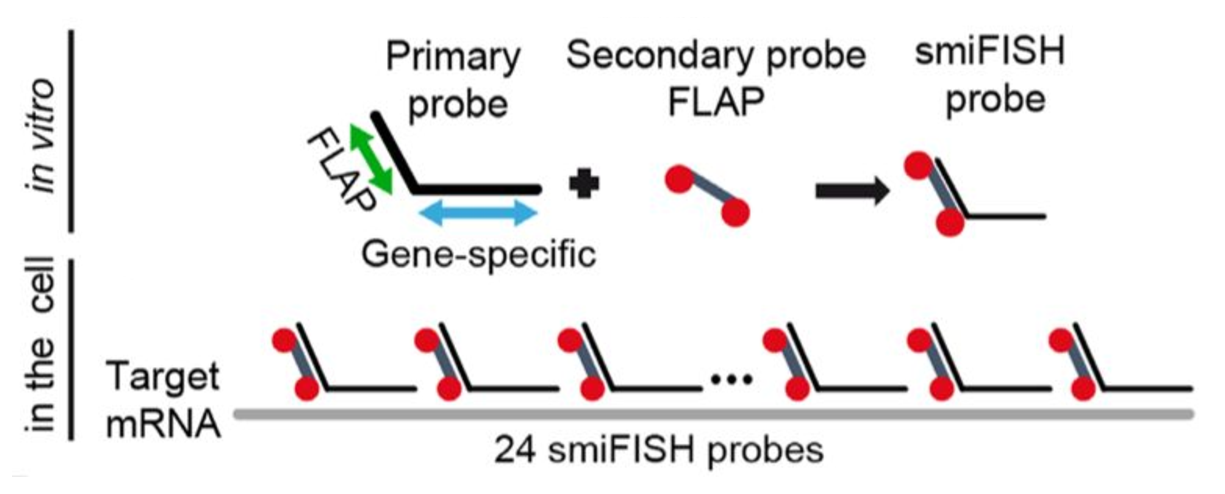
\includegraphics[width=\linewidth]{figures/introduction/smiFISH}
	\caption[Schema of smiFISH protocol]{Schema of smiFISH protocol from~\cite{tsanov_smifish_2016}}
	\label{fig:smiFISH}
	\end{center}
\end{wrapfigure}

In~\cite{tsanov_smifish_2016}, a cheaper and simpler version of \ac{smFISH} is presented: \ac{smiFISH}.
The fluorescent probe is built through a pre-hybridization step that matches a primary (unlabeled) probe with a secondary fluorescent oligonucleotide (see Figure~\ref{fig:smiFISH}).
This design with indirect labeling presents a higher flexibility and saves cost.
%Indeed, the fluorescent oligonucleotide can be generic while several specialized primary probes can target the \ac{RNA} molecule.

\subsection{Scaling up FISH}
\label{subsec:intro_scale_fish}

\begin{center}
	\textit{(To be completed)}
\end{center}



%Such indirect labeling techniques is also observed with more complex designs.



% indirect labelling (smifish, bDNA)

%- large scale screen (lecuyer, battich)
%- Merfish
%- seqfish
%- seqfish+

%\newacro{SeqFISH}{Sequential FISH}
%\newacro{MERFISH}{Multiplexed Error-Robust FISH}

%~\cite{lecuyer_global_2007} first large screen

%~\cite{Hedlund_2018} single cells RNA sequencing
%~\cite{bustin_absolute_2000} qRT-PCR
%~\cite{Hedlund_2018}
%~\cite{Hedlund_2018}
%~\cite{Hedlund_2018}
%~\cite{Femino_1998}




%Nevertheless, these techniques are witnessing rapid improvements in specificity, robustness, multiplexity, and background suppression.

%The first high-throughput mRNA localization screen was done in Drosophila embryos using whole mount FISH (LÈcuyer et al., 2007).

%%%%%%%%%%%%%%%%%%%%%%%%%%%%%%%%%%%%%%%%%%%%%%%%%%%%%%%%%%%%%%%%%%%%%%%%%%%%%%%%%%%%%%%%%%%%%%%%%%%%%%%%%%%%%%%%%%%%%%%%%%%%%%%%%%%%%%%%%%%%%%%%%%%%%%%%%%%%

% thesis adham: "the invention of single molecule FISH (Femino et al., 1998)"
% ~\cite{Femino_1998}

%%%%%%%%%%%%%%%%%%%%%%%%%%%%%%%%%%%%%%%%%%%%%%%%%%%%%%%%%%%%%%%%%%%%%%%%%%%%%%%%%%%%%%%%%%%%%%%%%%%%%%%%%%%%%%%%%%%%%%%%%%%%%%%%%%%%%%%%%%%%%%%%%%%%%%%%%%%%

% paper racha (dual protein-rna localization screens)

% In order to simultaneously visualize mRNAs with their encoded proteins, we based our screen on a library of HeLa cell lines,
% each containing a bacterial artificial chromosome (BAC) stably integrated in their genome (Poser et al., 2008).
% Each BAC con- tains a GFP-tagged gene harboring all its regulatory sequences (promoter, enhancers, introns, and 50 and 30 UTRs; Figure 1A).
% The resulting mRNAs are, thus, identical to the endogenous mol- ecules in terms of sequence and isoform diversity, except for the added tag.
% Previous studies showed that such tagged genes are expressed at near endogenous levels and with the proper spatio- temporal pattern (Poser et al., 2008).
% Since the tagged mRNAs contain all the regulatory sequences, we hypothesized that they would localize like the endogenous ones,
% provided that the tag does not interfere with localization. Using BACs offers two advantages. First, a single smFISH probe set
% against the GFP sequence is sufficient to detect all the studied mRNAs. Sec- ond, using mild hybridization conditions,
% GFP fluorescence can be detected together with the smFISH signal (Fusco et al., 2003), and thus, both the mRNA and the encoded protein can be detected in the same cell.

%%%%%%%%%%%%%%%%%%%%%%%%%%%%%%%%%%%%%%%%%%%%%%%%%%%%%%%%%%%%%%%%%%%%%%%%%%%%%%%%%%%%%%%%%%%%%%%%%%%%%%%%%%%%%%%%%%%%%%%%%%%%%%%%%%%%%%%%%%%%%%%%%%%%%%%%%%%%



%%%%%%%%%%%%%%%%%%%%%%%%%%%%%%%%%%%%%%%%%%%%%%%%%%%%%%%%%%%%%%%%%%%%%%%%%%%%%%%%%%%%%%%%%%%%%%%%%%%%%%%%%%%%%%%%%%%%%%%%%%%%%%%%%%%%%%%%%%%%%%%%%%%%%%%%%%%%
%%%%%%%%%%%%%%%%%%%%%%%%%%%%%%%%%%%%%%%%%%%%%%%%%%%%%%%%%%%%%%%%%%%%%%%%%%%%%%%%%%%%%%%%%%%%%%%%%%%%%%%%%%%%%%%%%%%%%%%%%%%%%%%%%%%%%%%%%%%%%%%%%%%%%%%%%%%%
%%%%%%%%%%%%%%%%%%%%%%%%%%%%%%%%%%%%%%%%%%%%%%%%%%%%%%%%%%%%%%%%%%%%%%%%%%%%%%%%%%%%%%%%%%%%%%%%%%%%%%%%%%%%%%%%%%%%%%%%%%%%%%%%%%%%%%%%%%%%%%%%%%%%%%%%%%%%

\section{Measuring images: from pixels to numbers}
\label{sec:computation_biology}

\subsection{Working with bioimages}
\label{subsec:intro_bioimages}

Recent developments in life sciences and technological breakthroughs greatly increase the importance of quantitative approaches.
A typical example is the Human Genome Project~\cite{lander_initial_2001} that aims to decipher human genome by the use of novel sequencing techniques.
Data collection and maintenance, as well as development of methods to extract valuable insights from it, is transforming biology in depth.
Current experimental platforms allow us to perform a large number of experiments under varied conditions and highly informative content.
These techniques are referred as High Content Screening and pave the way for a systematic analysis of living systems.
Finally, the increasing degree of automation of experimental protocols justifies the development of bioinformatics as a discipline in its own right to assist biologists.

The use of images in biology brings several advantages.
It enables the study of morphological patterns that could subsequently be related to phenotypes.
It also preserves the spatial dimension of the living system studied, as well as its temporal dimension in the case of repeated image acquisitions or live imaging experiments.
Last but not least, an analysis can be performed at different scales, from the molecule to the whole organ, through the tissues.
Overall, the tasks addressed with these bioimages can be
In general, the tasks performed with these bioimages can be as varied as the visualization of a living system, the reconstruction of a microscopy images, its denoising or the recognition of specific phenotypes.

One word to summarize bioimages would be \emph{heterogeneity}.
A living system can be imaged at different scales, with different modalities of acquisition and evolving technology.
In addition, the fluorescent markers used in microscopy or the question investigated by researcher could differ, making images of the same object from two different studies not necessarily compatible.
As a consequence, the subsequent computational analysis should be adapted for one set of images to another.

\subsection{Machine learning for bioimages}
\label{subsec:intro_ml_tools}

\subsubsection{A machine learning boom}

The recent years have seen a renewed interest for machine learning research, the cornerstone of current artificial intelligence era, driven by successful applications in vision, language understanding, speech recognition, etc\dots
This term of machine learning was coined to describe the set of techniques and models that make automatic decision based on patterns \emph{learned} and found in data.
For some specific tasks (like image classification) these algorithms have reached human-like capabilities.
For other fields, the gap between computer and human performances keeps decreasing.
In computer vision, the success of machine learning models makes their use legitimate for bioinformatics applications.\\

\noindent
Overall, three ingredients make these successes possible:
\begin{enumerate}
	\setlength\itemsep{0.1em}
	\item models fitted with learning algorithms
	\item large annotated datasets
	\item increased computing power to process an ever growing number of operations
\end{enumerate}

\noindent
The first ingredient is not necessarily new.
Machine learning and deep learning models (a family of machine learning models based on artificial neural networks), as well as learning algorithms have been studied and developed for decades (see~\cite{Bishop_2006, Tibshirani_2009} for a review of different machine learning methods).
As a symbol, the release of a large dataset with manual annotations for natural image classification problem~\cite{Deng_2009}, followed by a breakthrough performance with a \ac{CNN}~\cite{alexnet_2012}, marks the beginning of a new era for deep learning.
Obviously, the impact of these models has been consequent for every computational field.
In biomedical community, machine learning techniques are disseminating and address more challenges every year (see~\cite{jumper_highly_2021} for an example with the protein folding problem).

\subsubsection{Neural networks as the next generation tool}

In case of deep learning, model architecture is based on a neural network with successive layers of artificial neurons.
Each neuron is defined by a set of weights and perform a linear combination of the input signal with its weights, followed by a potential non linear transformation (usually a \emph{maxout}, \emph{sigmoid} or \emph{tanh} function).
A complete network usually combines these layers of neurons with normalization steps.
It can be seen as a parametrized model, whose weights need to be optimized to minimize for a specific task.

Given an input, a loss function enables to compare the output signal of the model with a ground truth (the expected output signal) and thus compute a gradient (the first order derivative of the loss function).
The backpropagation of this gradient to the rest of the network makes it possible to update the weights of the layers in order to minimize the loss~\cite{rumelhart_learning_1986}.
This process defines a training step.
After several iterations, the loss and the gradient should decrease, and the network progressively stabilizes its weights.
The weights are ultimately frozen and the model is trained.

Such architecture is highly flexible and different variants have been developed, with convolutional or recurrent layers to name a few~\cite{lecun_deep_2015}.
For a general introduction to deep learning techniques, one can refer to~\cite{Goodfellow_2016}.

\subsubsection{Limitations and caveats}

Beyond the great performances returned by machine learning models, a number of limitations and caveats should be consider.

First, they require annotated datasets to train and evaluate the models.
Compare to natural images, this ground truth is particularly costly to obtained with biomedical images as it often involves the assignation of experts (medical doctor or biologists) to a time-consuming, repetitive and annoying task.
As a consequence, datasets available for a given biomedical problem are often too small, highly diversified or released without any useful manual annotations.

Second, machine learning algorithms require robust evaluation protocol, strong benchmarks and a rigorous choice of evaluation metrics\footnote{One can see~\cite{varoquaux_machine_2022} for a description of these evaluation caveats when machine learning models are applied to medical images.}.
It is necessary to prevent data leakage and firmly separate the train set from the test set in our dataset, otherwise models overfit to the training samples and badly generalize to unknown data.
If the test set is not representative of the data distribution, or too small, the evaluation will be biased and hardly reproducible~\cite{Varoquaux_cv_2018}.
Obviously, all these limitations are worsen by the inherent heterogeneity of bioimages and the difficulty to assemble manual annotations.
Working with machine learning models, one needs strong and diversified baselines that reflect the state-of-the-art of performances, as well as the right choice of metrics to compare his methods to the rest of the literature.

Third, flexibility of some models comes at a price: a sensitivity to the selected hyperparameters, which makes the evaluation all the more important.

Last but not least, most of the deep learning models appear like a black box solution with an internal process that cannot be easily or directly interpreted.
If this problem is more critical for direct medical applications than biological ones, yet it requires an important pedagogical effort to diffuse deep learning techniques to the rest of the scientific community.

\section{Goals and contributions}
\label{sec:contributions}

\subsection{Goals}
\label{subsec:intro_goals}

\begin{figure}[]
	\centering
	\minipage{0.2\textwidth}
		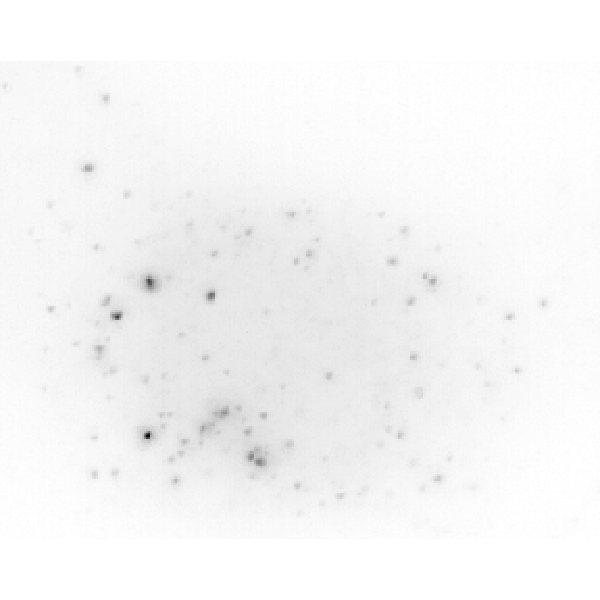
\includegraphics[width=0.95\linewidth]{figures/introduction/real_image_foci}
		\vfill
		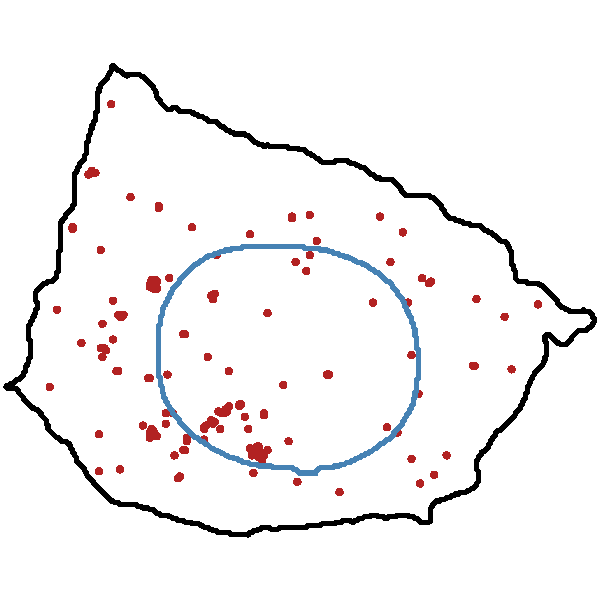
\includegraphics[width=0.95\linewidth]{figures/introduction/real_coord_foci}
		\subcaption{Foci}
	\endminipage\hfill
	\minipage{0.2\textwidth}
		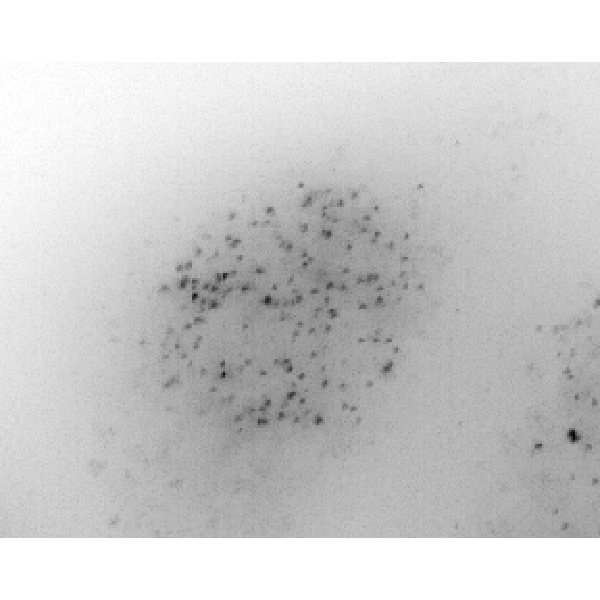
\includegraphics[width=0.95\linewidth]{figures/introduction/real_image_intranuclear}
		\vfill
		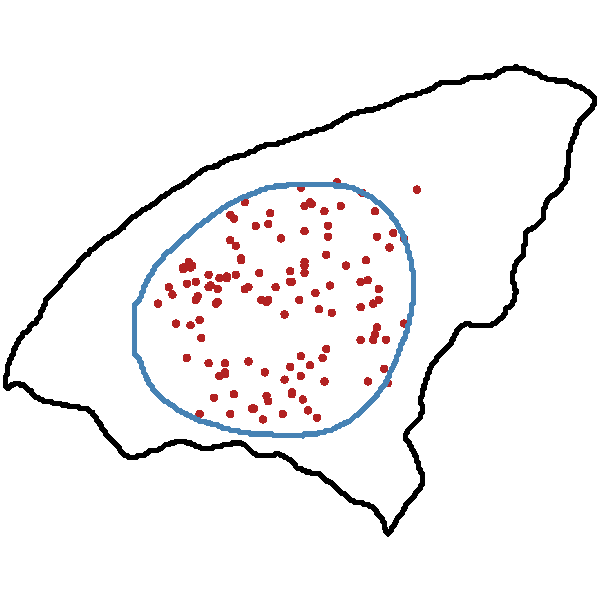
\includegraphics[width=0.95\linewidth]{figures/introduction/real_coord_intranuclear}
		\subcaption{Intranuclear}
	\endminipage\hfill
	\minipage{0.2\textwidth}
		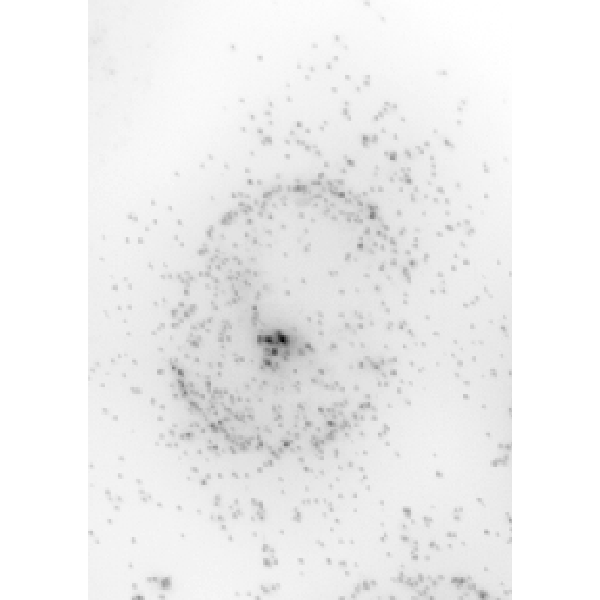
\includegraphics[width=0.95\linewidth]{figures/introduction/real_image_nuclear_edge}
		\vfill
		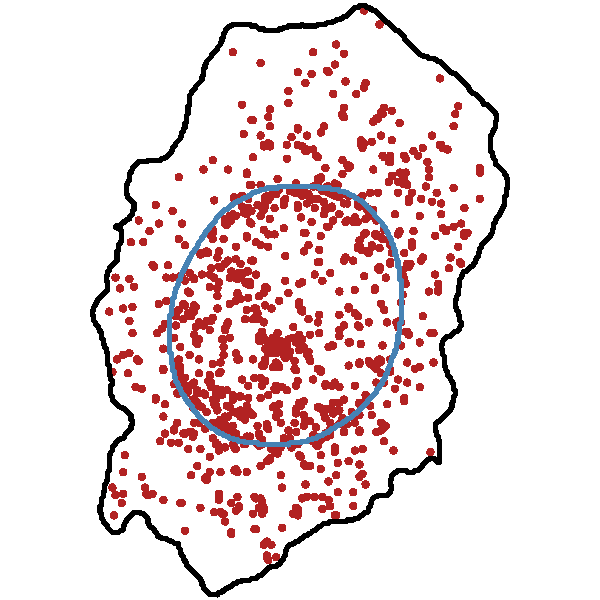
\includegraphics[width=0.95\linewidth]{figures/introduction/real_coord_nuclear_edge}
		\subcaption{Nuclear edge}
	\endminipage\hfill
	\minipage{0.2\textwidth}
		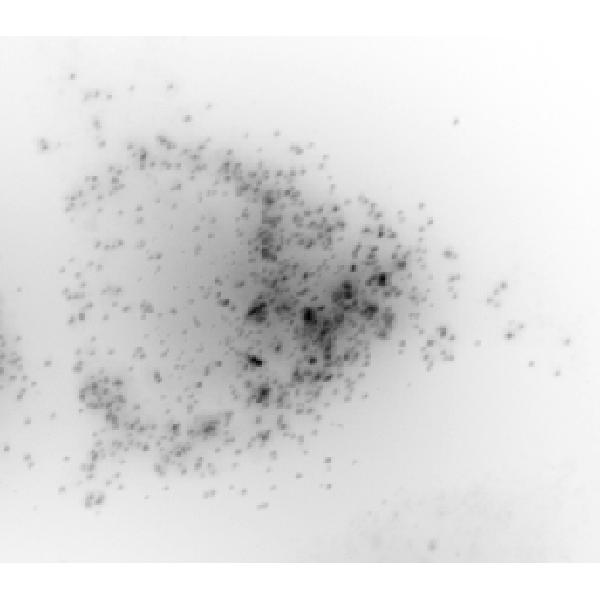
\includegraphics[width=0.95\linewidth]{figures/introduction/real_image_perinuclear}
		\vfill
		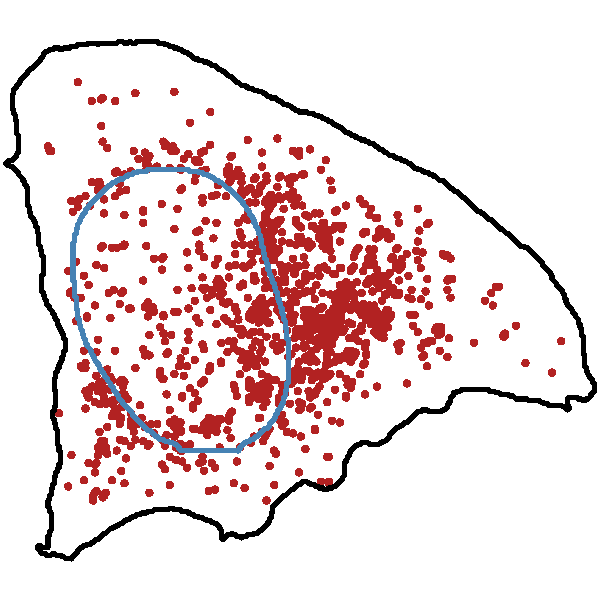
\includegraphics[width=0.95\linewidth]{figures/introduction/real_coord_perinuclear}
		\subcaption{Perinuclear}
	\endminipage\hfill
	\minipage{0.2\textwidth}
		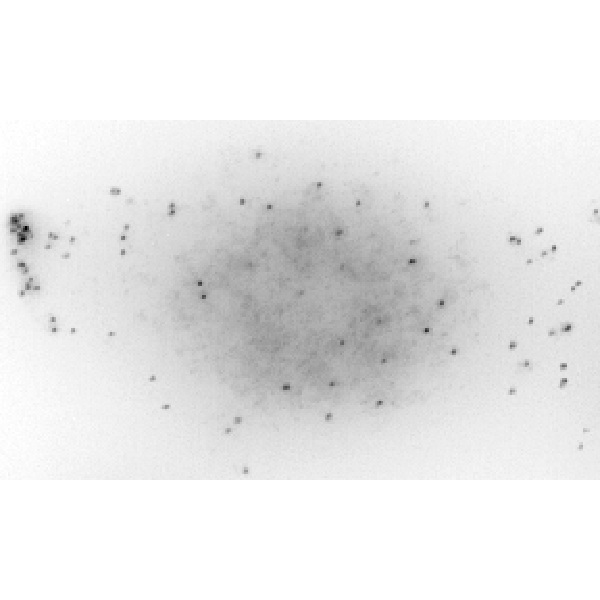
\includegraphics[width=0.95\linewidth]{figures/introduction/real_image_protrusion}
		\vfill
		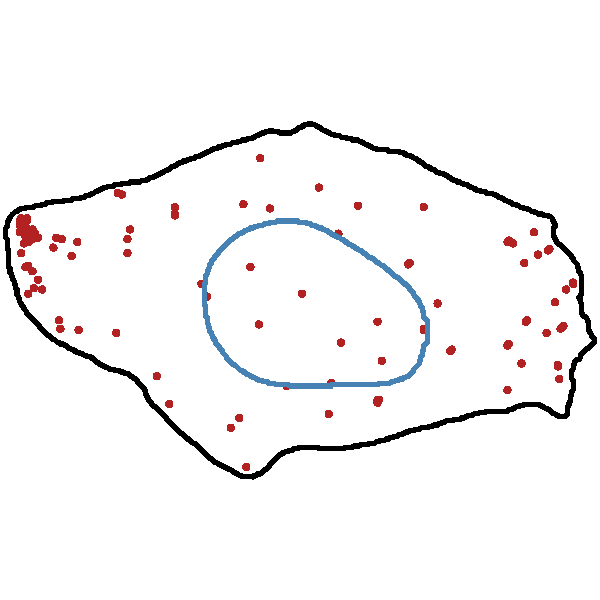
\includegraphics[width=0.95\linewidth]{figures/introduction/real_coord_protrusion}
		\subcaption{Protrusion}
	\endminipage
	\caption[RNA localization patterns from pixels to numbers]{RNA localization patterns from~\cite{pointfish_2022}.
	(\textit{Top}) Typical smFISH images with different RNA localization patterns.
	(\textit{Bottom}) Coordinate representations with RNA spots (\textit{red}), cell membrane (\textit{black}) and nuclear membrane (\textit{blue}).
	Detection and segmentation results are extracted and visualized with FISH-quant~\cite{Imbert_fq_2022}}
	\label{fig:intro_localization_patterns}
\end{figure}

At the beginning of my PhD, three main goals were defined with my supervisors.
The first one was the development and the implementation of a complete pipeline to process \ac{smFISH} images and return valuable insights about \ac{RNA} localization.
In particular, it was expected to integrate and adapt the latest successful developments in computer vision.
Figure~\ref{fig:intro_localization_patterns} illustrates the gap that needs to be bridged between the input images and an adequate representation of the \ac{RNA} localization, making their quantitative analysis possible.
The second goal was the identification of bottlenecks that would prevent scaling the analysis to thousands images, in high content screening assays.
Such bottlenecks should be minimized or solved during the thesis to be able to scale any computational analysis based on \ac{smFISH} experiments.
Lastly, this complete framework would be applied to real experimental datasets in ongoing biological studies.

\subsection{Contributions}
\label{subsec:intro_contributions}

Beyond this own manuscript, my contributions are essentially lines of code.
With a effort of transparency, reproducibility and documentation, I try to develop computational tools as useful as possible for any biologist interested in \ac{FISH} experiments.
My PhD results in three major contributions.

\begin{itemize}
	\setlength\itemsep{0.1em}
	\item My first and main contribution is FISH-quant V2.
	This online framework gathers Python packages and a \ac{GUI} to process \ac{FISH} images, build robust analysis pipelines and even perform simulations.
	\item My second important contribution is an alternative method to compute relevant features in order to discriminate \ac{RNA} localization patterns.
	This method implies the development of PointFISH, a dedicated deep learning model for point cloud.
	\item My third contribution is my participation to biological studies with meaningful results.
	These studies leveraged high content screening assays and \ac{smFISH} techniques to perform a systemic analysis of \ac{RNA} localization and investigate local translation phenomenons.
\end{itemize}

\noindent
Some other contributions are also mentioned throughout this manuscript.
It includes a dataset I annotated for nucleus and cell segmentation with thousands of instances and my supervision of an intern.
The work performed during this internship was the seed for the first publication of another PhD student in the team, about in silico labeling and segmentation.
Lastly, a list of my publications are available at the very end of the manuscript.

\subsection{Manuscript summary}
\label{subsec:intro_manuscript}

The manuscript is composed of two parts.
The first four chapters are a presentation of the analysis pipeline with a focus on every critical stage.
It includes systematic reviews of the existing methods and details about solutions I implemented.
In addition, code snippets, ready to be imported and run, are interspersed with descriptions of the related algorithms.
The second part details several applications of my tools, where quantification of \ac{RNA} localization patterns supports biological insights.

In \textbf{Chapter~\ref{ch:chapter1}}, I present the general computational framework I developed and published: FISH-quant v2.
It includes methods for every stages of a \ac{FISH}-based analysis, with an effort to make them scalable and modular.
I also describe the improvements from the original FISH-quant version, and how it addresses the requirements of a modern software tool.

In \textbf{Chapter~\ref{ch:chapter2}}, I focus on the \ac{RNA} detection stage.
With \ac{smFISH} experiments, the \ac{RNA} molecules are spotted and reduced to discrete data points in space.
I describe detection algorithms and their extensions available in FISH-quant.
In the end, the set of all \ac{RNA} molecules is reduced to a point cloud with spatial coordinates.

In \textbf{Chapter~\ref{ch:chapter3}}, I review and describe algorithms for nucleus and cell segmentation.
Most of them are deep learning models, trained on vast datasets of annotated images.
Beside my own implemented methods, I also present refinement techniques to improve and format segmentation masks.
Two other projects for which I contributed (including one published) are also discussed at the end of the chapter.
They aim at improving the efficiency and consistency of segmentation on specific aspects.

In \textbf{Chapter~\ref{ch:chapter4}}, I compare two different approaches to quantify \ac{RNA} localization patterns.
Once the \ac{RNA} molecules are detected and cell morphology is segmented, the pixel domain gives way to Euclidean space and cells can be represented with a coordinate representation.
Then, spatial features are computed in order to discriminate relevant localization pattern.
I present two different methods of feature engineering.
The first method consists in manually designing features to characterize specific localization patterns.
I then list and describe every hand-crafted feature implemented in FISH-quant.
The second (published) method consists in learning features.
They are extracted from a deep learning model fed with the \ac{RNA} point cloud as input and trained on a simulated pretext task.

In \textbf{Chapter~\ref{ch:chapter5}}, I present several applications of my quantitative pipeline.
These applications come from three publications where we study different \ac{RNA} localization patterns and cases of local translation.
My analyses support and validates biological insights claimed in these studies about \ac{RNA} localization.
I design a classification pipeline to recognize generic localization patterns.
I evaluate the impact of translation inhibitor on \ac{RNA} localization and help identifying a singular translation-dependent pattern.
I quantify a cell cycle dependent pattern, which is related to centrosomes.
Finally, I also contribute to a a study focused on the protrusion pattern.
